\chapter{Realisation of a demonstrator}
%\textbf{keep it small and simple} 
%Outline of the technologies used to fabricate and assemble your structures, if applicable. Detailed processes belong in the appendix. If numerous types of structures were fabricated, or assembly technology is extensive, there may be more than one of these chapters. \textbf{Characterization} Description of the means developed and employed to characterize the devices or systems that have been fabricated.
%The realisation of the demonstrated concepts on a hybrid substrate was one goal of this thesis, to show its feasibility.
The demonstrator consists of several (multi assembled) \gls{ab:mmic} chips with a filter network built by discrete \gls{ab:smd} decoupling capacitors.
Therefore the realised demonstrator is a hybrid test circuit.
To avoid building a too complex structure the resolution of the \gls{ab:dac} was restricted to two bit.
With two bit resolution there are already four inputs which need to be controlled via a high speed digital signal.
In order to ensure that the \gls{ab:hemt} base transistor at the input of the circuit is fully switched on and off a peak to peak value of \SI{5}{\volt} is needed.
%\SI{5}{\volt} peak to peak input signal is needed to ensure that the \gls{ab:hemt} is fully opened or fully closed. 
If a third bit of resolution was added this would increase the number of inputs to six, which makes the circuit and the test setup more complex.
\\
A two layer high frequency roger substrate, namely Rogers 4003, is used.
Rogers 4003 substrates have nice properties with respect to high frequency applications.
The dissipation factor is 0.0027, while dielectric constant is 3.55 and thermal coefficient is +40. % which parameters are really helpfull in contrast to other materials?
Two different designs were ordered both with a \SI{35}{\micro \metre} Cu conduction layer, ChemNiPdAu metallisation and a thickness of \SI{0.508}{\milli \metre}.
An impedance control of the \SI{50}{\ohm} input lines as well for the \SI{50}{\ohm} output line is performed by the manufacturer, Contag AG, to ensure the best matching.
\\
The different version are designed with the background of using different chips with different properties.
One layout is designed for chips which backside metallization is grounded with vias.
To realize a high side switch with those chips, they have to be put on a pad without gnd contact.
The source contact of the chip is the output for the high side, while the source contact of the lowside switch is grounded.
Therefore for the lowside the chips is mounted on the ground layer.
Chips with this properties are designed by Stephan Maroldt, namely DDRi\_X6 and DDRi\_Y6.\\
The other version of the designed substrate is for chips, which backside metallization is not connected to the chips "GND" potential with vias.
Therefore this version could be mounted (soldered) to the conduction layer without the need of an isolated pad.
These chips DDRi\_2C, also designed by Stephan Maroldt, have to be bonded to the substrate GND separately.



\section{Substrate layout using DDRi\_X6 and DDRi\_Y6 chips}
%\begin{enumerate}
%	\item Highside driver load transistor voltage connected to Vdd
%	\item Highside driver load transistor voltage connected to Vout
%\end{enumerate}

The presented layout of the substrate is designed for the use of the chips DDRi\_X6 and DDRi\_Y6.
Figure \ref{fig:layoutDDRiXY6sub} shows an overview of the designed layout.

\begin{figure}[htb!]
	\centering
  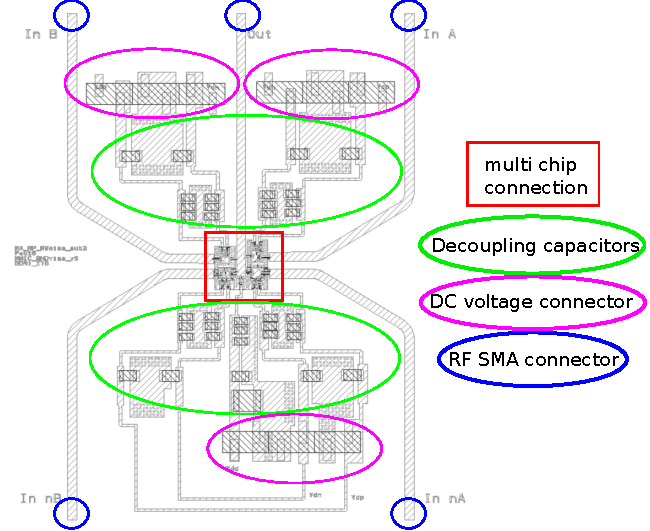
\includegraphics{Layout_DDRiXY6_new_grey.pdf}
	\caption{Layout substrate with DDRi\_XY6 chips}
	\label{fig:layoutDDRiXY6sub}
\end{figure}

It is to mention that the part outside the red marked rectangular box of this layout is nearly identical for the other design version.
Only one additional \gls{ab:dc} voltage supply line and a different arrangement of the chips is considered.
The described part outside the red box consists of the \gls{ab:smd} decoupling capacitor filter network and the multi pin connector for the \gls{ab:dc} voltage supply.\\
The filter network consisting of several decoupling capacitors is designed by the right choice of capacitors.
The very first decoupling capacitor is integrated in the chip, while the second is a special \gls{ab:mmic} capacitor mounted on the backside connected layer.
The purpose of the bypass capacitors were to filter out undesired distortion frequencies which could lead to oscillation of the circuit.
A few bypass capacitors are used based on the experience and experimental advice of some colleagues, rule of thumb. 
Suitable capacitors were those with a high \gls{ab:esr} which means a bad q-factor, and of course the temperature range, the voltage range should be suitable to the purpose(flatten mag of imp vs. freq broadband good).
(Bypassing and operating frequency not necessarily linked to each other. Bypassing a greater range than the potential operating frequency) (Culture Cargo principle). 
The first bypass capacitance the chip supply voltage sees is a MMIC cap directly assembled near to the supply pin of the chip.
The values of the used capacitors in the order of placement starting at the chip supply in the middle of the substrate (82p, 1n, 10n, 100n, 1u, 10u (only Vdd)).
This undesired distortion frequencies could make the circuit unstable.\\
The size of the used pads for the GND potential is designed larger than necessary to make it easier to change the capacitors.
The GND potential pads also have some via holes in fact that more via holes could make the thermal dissipation only better than worse.\\
The four input lines as well as the output line were designed to have an impedance of \SI{50}{\ohm} to ensure matching to the cables for the measurement.\\
Distance between conduction layer is limited by the processing steps of the manufacturer.
In the layout process it was kept in mind to reduce the capacitive coupling between supply and signal lines.\\
The assembly of the multi chip connection marked with the red rectangular is described in Figure \ref{fig:layoutDDRiXY6bond}.

\begin{figure}[htb!]
	\centering
  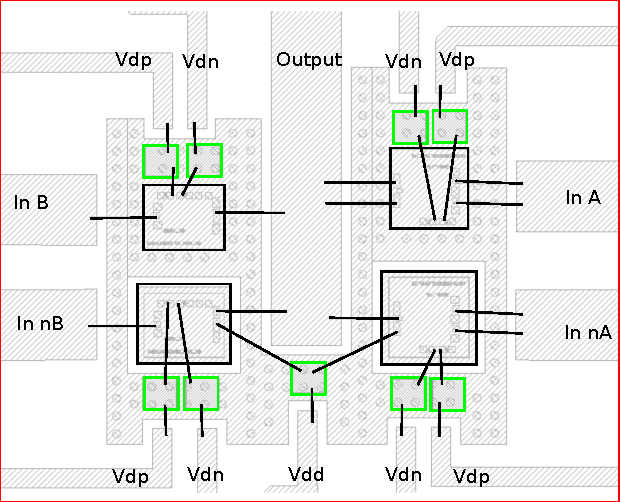
\includegraphics{Layout_DDRiXY6_bonds_new.pdf}
	\caption{Layout DDRi\_X6 and DDRi\_Y6 chips}
	\label{fig:layoutDDRiXY6bond}
\end{figure}

One very important design rule for this layout was to create as much as possible heat transfer.
The drawback of the chosen chips were that in fact of the backside metallization and their via hole to the backside, this chips had to be placed on an isolated pad.
In Figure \ref{fig:layoutDDRiXY6bond} the chips at the bottom marked (black)  were placed on an isolated pad.
This pad did not have any connection to the GND potential of the substrate.
The pad were placed in the near of a conducting layer with via holes to spread the heat over the air bridge (ambient temperature) through the via hole to the backside. 
This isolation pad had to be established since these chips were switched at the high-side to provide Vdd to the output. 
Due to the assembling on an isolated pad, the heat transfer is much worse than for the other chips.
This is not the optimal way to dissipate the heat, but the only to handle some heat dissipation.
This is a very critical design issue since the chips create much heat.
A pad which is surrounded by the back sided conductive layer was used to enable at least some heat transfer to the backside of the demonstrator.
Since there was no other option to dissipate the heat in this configuration this was the chosen approach.\\
The length of the bond wires, were set to be equal for the critical signal paths of the in- and output connection.
Since an in-phase control of the input was important to ensure the switches to turn on/off synchronous.
The length of the bond wires providing the \gls{ab:dc} voltage supply were not critical.
The diameter of the wedged \gls{ab:au} bond wire was set to \SI{25}{\micro \metre} which ensured a maximum current of approximated \SI{1}{\ampere} for a bond length of \SI{1}{\milli \metre}.
The small diameter and the short length made it most suitable for the high frequency application.\\
A first mounted decoupling capacitor were a \SI{82}{\pico \farad} \gls{ab:smd} ceramic capacitor, namely D20BT820K5PX from Dielectric Laboratories Inc.\textbf{attach Datasheet?}.
The gold metallization (for wire bonding), the thin film technology and the custom sizes (to keep it small), made this the most suitable capacitor for the purpose of \gls{ab:dc} blocking.





\section{Substrate layout using DDRi\_2C chips}
As mentioned before the layout of the filter network and the dc supply voltage did not differ as much from the other layout version.
In this version an additional connector is applied to provide one additional dc supply voltage.
Furthermore the arrangement of the chips is different.
Figure \ref{fig:layoutDDRi2Cbond} shows the arrangement of the used chips, namely DDRi\_2C designed by Stephan Maroldt.

\begin{figure}[htb!]
	\centering
  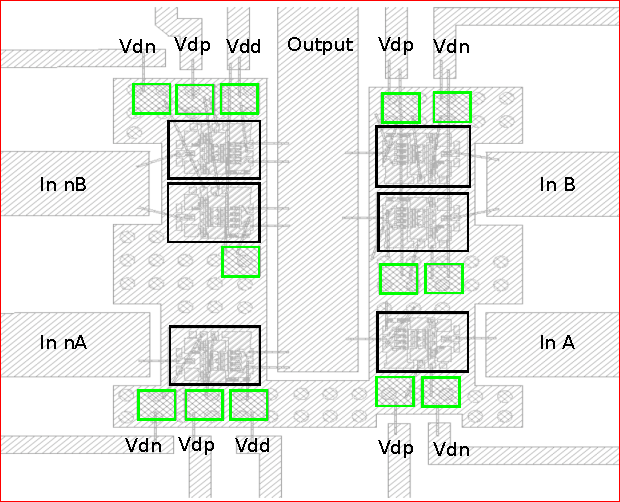
\includegraphics{Layout_DDRi2C_bonds.pdf}
	\caption{Layout DDRi\_2C chips}
	\label{fig:layoutDDRi2Cbond}
\end{figure}

The important difference between the DDRi\_2C chips and DDRi\_X6/DDRi\_Y6 is, that the DDRi\_2C chips do not have a connection to their backside.
Hence this chips could be directly soldered to the grounded backside connection of the layer.
The heat could spread directly from the backside of the chip which is metallized through the via holes of the substrate to the substrates backside.
In fact of this, the heat transfer is much better than of the other design.
In contrast to the other version, it is important that the gnd pads of the chip are bonded onto the substrate GND potential. 
This version could be more convenient due to the better heat dissipation.\\

\section{Evaluation of the design and realisation process}
In the realisation and layout process many things must be considered.\\
The circuit is build on a hybrid assembly which combines the MMIC with the discrete SMD components on a Rogers 4003 substrate.\\
The input and output lines on the substrate were \gls{ab:msl} which were matched to \SI{50}{\ohm}.
%Tuned in this sense means, the lines were created with the right width, length and depth on the correct substrate with a special thickness.
Important for the design of the input lines were that they are of the same length, due to timing issues.
The input timing is crucial due to the fact that the switches have to switch synchronous.
The output line was matched to \SI{50}{\ohm} to ensure proper measuring.\\
%Also it would tried to get a proper distance between the lines to avoid any coupling. \\
In addition to the same length of the input lines, also the bond wires of the in- and output to the \gls{ab:mmic} chips should be of the same length.
 %The idea is that the high frequency digital signal are not allowed to have phase angles, because the switches have to switch all at the same time. Timing problems are expected to occur within the measurement. \\
One of the most important and crucial things is the generation of heat which had to be dissipated.
Based on the designed chips, two different concepts were chosen to dissipate the heat in the most proper way.\\
The wafer run of the chips DDRi\_2C is from the year 2011 and therefore five years old and hence the taping of the wafer could be not as good as the newer ones.
\\
Due to this heat dissipation problem it was then that it renounces to package the chips into a \gls{ab:qfn} package.\\
For bonding \SI{25}{\micro \metre} (diameter) \gls{ab:au} bonds were used.
The length of the bonds were given by assembly limits for spacing of conducting layers  due to manufacturer process limits.\\
In- and output connectors were commercially available SMA jack connectors with a matched impedance of \SI{50}{\ohm} to connect standard RF cables.\\

%Capacitive coupling could be a problem, through the dc supply lines to the input lines.
%What about the coupling from the substrate backside to the conducting layer of the substrate? 
%What about inductive coupling via the via holes or so??
%Other coupling?\\

The two layouts were fabricated by CONTAG AG while the needed components were ordered at Digi-Key Electronics.\\
The finished demonstrator is shown in Figure \ref{fig:assembledDemonstrator}with a short description of the placed elements.

\begin{figure}[htb!]
	\centering
  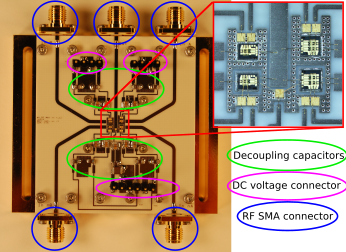
\includegraphics{Demonstrator_edited_newScale.pdf}
	\caption{Assembled demonstrator}
	\label{fig:assembledDemonstrator}
\end{figure}

\begin{figure}[htb!]
	\centering
  \includegraphics{ComparePhotoXY6_2C.pdf}
	\caption{Comparison of assembled chips DDRi\_X6 \& DDRi\_Y6 (left) and DDRi\_2C (right)}
	\label{fig:CompareChips}
\end{figure}
